\documentclass[1p]{elsarticle_modified}
%\bibliographystyle{elsarticle-num}

%\usepackage[colorlinks]{hyperref}
%\usepackage{abbrmath_seonhwa} %\Abb, \Ascr, \Acal ,\Abf, \Afrak
\usepackage{amsfonts}
\usepackage{amssymb}
\usepackage{amsmath}
\usepackage{amsthm}
\usepackage{scalefnt}
\usepackage{amsbsy}
\usepackage{kotex}
\usepackage{caption}
\usepackage{subfig}
\usepackage{color}
\usepackage{graphicx}
\usepackage{xcolor} %% white, black, red, green, blue, cyan, magenta, yellow
\usepackage{float}
\usepackage{setspace}
\usepackage{hyperref}

\usepackage{tikz}
\usetikzlibrary{arrows}

\usepackage{multirow}
\usepackage{array} % fixed length table
\usepackage{hhline}

%%%%%%%%%%%%%%%%%%%%%
\makeatletter
\renewcommand*\env@matrix[1][\arraystretch]{%
	\edef\arraystretch{#1}%
	\hskip -\arraycolsep
	\let\@ifnextchar\new@ifnextchar
	\array{*\c@MaxMatrixCols c}}
\makeatother %https://tex.stackexchange.com/questions/14071/how-can-i-increase-the-line-spacing-in-a-matrix
%%%%%%%%%%%%%%%

\usepackage[normalem]{ulem}

\newcommand{\msout}[1]{\ifmmode\text{\sout{\ensuremath{#1}}}\else\sout{#1}\fi}
%SOURCE: \msout is \stkout macro in https://tex.stackexchange.com/questions/20609/strikeout-in-math-mode

\newcommand{\cancel}[1]{
	\ifmmode
	{\color{red}\msout{#1}}
	\else
	{\color{red}\sout{#1}}
	\fi
}

\newcommand{\add}[1]{
	{\color{blue}\uwave{#1}}
}

\newcommand{\replace}[2]{
	\ifmmode
	{\color{red}\msout{#1}}{\color{blue}\uwave{#2}}
	\else
	{\color{red}\sout{#1}}{\color{blue}\uwave{#2}}
	\fi
}

\newcommand{\Sol}{\mathcal{S}} %segment
\newcommand{\D}{D} %diagram
\newcommand{\A}{\mathcal{A}} %arc


%%%%%%%%%%%%%%%%%%%%%%%%%%%%%5 test

\def\sl{\operatorname{\textup{SL}}(2,\Cbb)}
\def\psl{\operatorname{\textup{PSL}}(2,\Cbb)}
\def\quan{\mkern 1mu \triangleright \mkern 1mu}

\theoremstyle{definition}
\newtheorem{thm}{Theorem}[section]
\newtheorem{prop}[thm]{Proposition}
\newtheorem{lem}[thm]{Lemma}
\newtheorem{ques}[thm]{Question}
\newtheorem{cor}[thm]{Corollary}
\newtheorem{defn}[thm]{Definition}
\newtheorem{exam}[thm]{Example}
\newtheorem{rmk}[thm]{Remark}
\newtheorem{alg}[thm]{Algorithm}

\newcommand{\I}{\sqrt{-1}}
\begin{document}

%\begin{frontmatter}
%
%\title{Boundary parabolic representations of knots up to 8 crossings}
%
%%% Group authors per affiliation:
%\author{Yunhi Cho} 
%\address{Department of Mathematics, University of Seoul, Seoul, Korea}
%\ead{yhcho@uos.ac.kr}
%
%
%\author{Seonhwa Kim} %\fnref{s_kim}}
%\address{Center for Geometry and Physics, Institute for Basic Science, Pohang, 37673, Korea}
%\ead{ryeona17@ibs.re.kr}
%
%\author{Hyuk Kim}
%\address{Department of Mathematical Sciences, Seoul National University, Seoul 08826, Korea}
%\ead{hyukkim@snu.ac.kr}
%
%\author{Seokbeom Yoon}
%\address{Department of Mathematical Sciences, Seoul National University, Seoul, 08826,  Korea}
%\ead{sbyoon15@snu.ac.kr}
%
%\begin{abstract}
%We find all boundary parabolic representation of knots up to 8 crossings.
%
%\end{abstract}
%\begin{keyword}
%    \MSC[2010] 57M25 
%\end{keyword}
%
%\end{frontmatter}

%\linenumbers
%\tableofcontents
%
\newcommand\colored[1]{\textcolor{white}{\rule[-0.35ex]{0.8em}{1.4ex}}\kern-0.8em\color{red} #1}%
%\newcommand\colored[1]{\textcolor{white}{ #1}\kern-2.17ex	\textcolor{white}{ #1}\kern-1.81ex	\textcolor{white}{ #1}\kern-2.15ex\color{red}#1	}

{\Large $\underline{12n_{0504}~(K12n_{0504})}$}

\setlength{\tabcolsep}{10pt}
\renewcommand{\arraystretch}{1.6}
\vspace{1cm}\begin{tabular}{m{100pt}>{\centering\arraybackslash}m{274pt}}
\multirow{5}{120pt}{
	\centering
	\includegraphics[width=112pt]{../../../GIT/diagram.site/Diagrams/png/2593_12n_0504.png}\\
\ \ \ A knot diagram\footnotemark}&
\allowdisplaybreaks
\textbf{Linearized knot diagam} \\
\cline{2-2}
 &
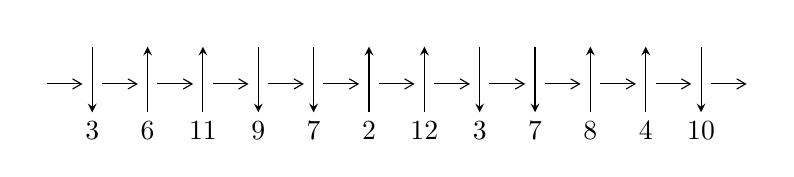
\begin{tikzpicture}[x=20pt, y=17pt]
	% nodes
	\node (C0) at (0, 0) {};
	\node (C1) at (1, 0) {};
	\node (C1U) at (1, +1) {};
	\node (C1D) at (1, -1) {3};

	\node (C2) at (2, 0) {};
	\node (C2U) at (2, +1) {};
	\node (C2D) at (2, -1) {6};

	\node (C3) at (3, 0) {};
	\node (C3U) at (3, +1) {};
	\node (C3D) at (3, -1) {11};

	\node (C4) at (4, 0) {};
	\node (C4U) at (4, +1) {};
	\node (C4D) at (4, -1) {9};

	\node (C5) at (5, 0) {};
	\node (C5U) at (5, +1) {};
	\node (C5D) at (5, -1) {7};

	\node (C6) at (6, 0) {};
	\node (C6U) at (6, +1) {};
	\node (C6D) at (6, -1) {2};

	\node (C7) at (7, 0) {};
	\node (C7U) at (7, +1) {};
	\node (C7D) at (7, -1) {12};

	\node (C8) at (8, 0) {};
	\node (C8U) at (8, +1) {};
	\node (C8D) at (8, -1) {3};

	\node (C9) at (9, 0) {};
	\node (C9U) at (9, +1) {};
	\node (C9D) at (9, -1) {7};

	\node (C10) at (10, 0) {};
	\node (C10U) at (10, +1) {};
	\node (C10D) at (10, -1) {8};

	\node (C11) at (11, 0) {};
	\node (C11U) at (11, +1) {};
	\node (C11D) at (11, -1) {4};

	\node (C12) at (12, 0) {};
	\node (C12U) at (12, +1) {};
	\node (C12D) at (12, -1) {10};
	\node (C13) at (13, 0) {};

	% arrows
	\draw[->,>={angle 60}]
	(C0) edge (C1) (C1) edge (C2) (C2) edge (C3) (C3) edge (C4) (C4) edge (C5) (C5) edge (C6) (C6) edge (C7) (C7) edge (C8) (C8) edge (C9) (C9) edge (C10) (C10) edge (C11) (C11) edge (C12) (C12) edge (C13) ;	\draw[->,>=stealth]
	(C1U) edge (C1D) (C2D) edge (C2U) (C3D) edge (C3U) (C4U) edge (C4D) (C5U) edge (C5D) (C6D) edge (C6U) (C7D) edge (C7U) (C8U) edge (C8D) (C9U) edge (C9D) (C10D) edge (C10U) (C11D) edge (C11U) (C12U) edge (C12D) ;
	\end{tikzpicture} \\
\hhline{~~} \\& 
\textbf{Solving Sequence} \\ \cline{2-2} 
 &
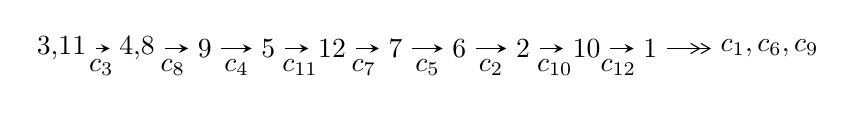
\begin{tikzpicture}[x=23pt, y=7pt]
	% node
	\node (A0) at (-1/8, 0) {3,11};
	\node (A1) at (17/16, 0) {4,8};
	\node (A2) at (17/8, 0) {9};
	\node (A3) at (25/8, 0) {5};
	\node (A4) at (33/8, 0) {12};
	\node (A5) at (41/8, 0) {7};
	\node (A6) at (49/8, 0) {6};
	\node (A7) at (57/8, 0) {2};
	\node (A8) at (65/8, 0) {10};
	\node (A9) at (73/8, 0) {1};
	\node (C1) at (1/2, -1) {$c_{3}$};
	\node (C2) at (13/8, -1) {$c_{8}$};
	\node (C3) at (21/8, -1) {$c_{4}$};
	\node (C4) at (29/8, -1) {$c_{11}$};
	\node (C5) at (37/8, -1) {$c_{7}$};
	\node (C6) at (45/8, -1) {$c_{5}$};
	\node (C7) at (53/8, -1) {$c_{2}$};
	\node (C8) at (61/8, -1) {$c_{10}$};
	\node (C9) at (69/8, -1) {$c_{12}$};
	\node (A10) at (11, 0) {$c_{1},c_{6},c_{9}$};

	% edge
	\draw[->,>=stealth]	
	(A0) edge (A1) (A1) edge (A2) (A2) edge (A3) (A3) edge (A4) (A4) edge (A5) (A5) edge (A6) (A6) edge (A7) (A7) edge (A8) (A8) edge (A9) ;
	\draw[->>,>={angle 60}]	
	(A9) edge (A10);
\end{tikzpicture} \\ 

\end{tabular} \\

\footnotetext{
The image of knot diagram is generated by the software ``\textbf{Draw programme}" developed by Andrew Bartholomew(\url{http://www.layer8.co.uk/maths/draw/index.htm\#Running-draw}), where we modified some parts for our purpose(\url{https://github.com/CATsTAILs/LinksPainter}).
}\phantom \\ \newline 
\centering \textbf{Ideals for irreducible components\footnotemark of $X_{\text{par}}$} 
 
\begin{align*}
I^u_{1}&=\langle 
1.23441\times10^{152} u^{80}+1.03277\times10^{152} u^{79}+\cdots+7.12803\times10^{149} b+1.45911\times10^{152},\\
\phantom{I^u_{1}}&\phantom{= \langle  }-1.08125\times10^{152} u^{80}-9.29614\times10^{151} u^{79}+\cdots+7.12803\times10^{149} a-1.25045\times10^{152},\\
\phantom{I^u_{1}}&\phantom{= \langle  }u^{81}-25 u^{79}+\cdots- u-1\rangle \\
I^u_{2}&=\langle 
- u^{19}- u^{18}+\cdots+b-1,\;-7529 u^{20}+16576 u^{19}+\cdots+4369 a+66551,\;u^{21}+u^{20}+\cdots+u-1\rangle \\
\\
\end{align*}
\raggedright * 2 irreducible components of $\dim_{\mathbb{C}}=0$, with total 102 representations.\\
\footnotetext{All coefficients of polynomials are rational numbers. But the coefficients are sometimes approximated in decimal forms when there is not enough margin.}
\newpage
\renewcommand{\arraystretch}{1}
\centering \section*{I. $I^u_{1}= \langle 1.23\times10^{152} u^{80}+1.03\times10^{152} u^{79}+\cdots+7.13\times10^{149} b+1.46\times10^{152},\;-1.08\times10^{152} u^{80}-9.30\times10^{151} u^{79}+\cdots+7.13\times10^{149} a-1.25\times10^{152},\;u^{81}-25 u^{79}+\cdots- u-1 \rangle$}
\flushleft \textbf{(i) Arc colorings}\\
\begin{tabular}{m{7pt} m{180pt} m{7pt} m{180pt} }
\flushright $a_{3}=$&$\begin{pmatrix}1\\0\end{pmatrix}$ \\
\flushright $a_{11}=$&$\begin{pmatrix}0\\u\end{pmatrix}$ \\
\flushright $a_{4}=$&$\begin{pmatrix}1\\- u^2\end{pmatrix}$ \\
\flushright $a_{8}=$&$\begin{pmatrix}151.690 u^{80}+130.417 u^{79}+\cdots+384.512 u+175.426\\-173.177 u^{80}-144.889 u^{79}+\cdots-450.511 u-204.700\end{pmatrix}$ \\
\flushright $a_{9}=$&$\begin{pmatrix}324.867 u^{80}+275.305 u^{79}+\cdots+835.023 u+380.126\\-173.177 u^{80}-144.889 u^{79}+\cdots-450.511 u-204.700\end{pmatrix}$ \\
\flushright $a_{5}=$&$\begin{pmatrix}-217.115 u^{80}-183.775 u^{79}+\cdots-589.240 u-262.760\\83.8333 u^{80}+71.1008 u^{79}+\cdots+215.196 u+102.506\end{pmatrix}$ \\
\flushright $a_{12}=$&$\begin{pmatrix}u\\- u^3+u\end{pmatrix}$ \\
\flushright $a_{7}=$&$\begin{pmatrix}303.584 u^{80}+259.429 u^{79}+\cdots+777.896 u+355.169\\-130.110 u^{80}-108.535 u^{79}+\cdots-338.033 u-153.969\end{pmatrix}$ \\
\flushright $a_{6}=$&$\begin{pmatrix}-290.200 u^{80}-249.523 u^{79}+\cdots-729.435 u-337.494\\85.7527 u^{80}+71.4068 u^{79}+\cdots+225.793 u+102.293\end{pmatrix}$ \\
\flushright $a_{2}=$&$\begin{pmatrix}-264.895 u^{80}-226.810 u^{79}+\cdots-666.097 u-306.595\\95.4427 u^{80}+78.6904 u^{79}+\cdots+251.393 u+112.450\end{pmatrix}$ \\
\flushright $a_{10}=$&$\begin{pmatrix}183.583 u^{80}+153.132 u^{79}+\cdots+480.308 u+219.882\\-72.9647 u^{80}-64.8472 u^{79}+\cdots-178.991 u-84.6969\end{pmatrix}$ \\
\flushright $a_{1}=$&$\begin{pmatrix}-169.452 u^{80}-148.120 u^{79}+\cdots-414.704 u-194.145\\95.4427 u^{80}+78.6904 u^{79}+\cdots+251.393 u+112.450\end{pmatrix}$\\&\end{tabular}
\flushleft \textbf{(ii) Obstruction class $= -1$}\\~\\
\flushleft \textbf{(iii) Cusp Shapes $= -134.434 u^{80}-107.850 u^{79}+\cdots-374.672 u-167.881$}\\~\\
\newpage\renewcommand{\arraystretch}{1}
\flushleft \textbf{(iv) u-Polynomials at the component}\newline \\
\begin{tabular}{m{50pt}|m{274pt}}
Crossings & \hspace{64pt}u-Polynomials at each crossing \\
\hline $$\begin{aligned}c_{1},c_{5}\end{aligned}$$&$\begin{aligned}
&u^{81}+48 u^{80}+\cdots-46 u-1
\end{aligned}$\\
\hline $$\begin{aligned}c_{2},c_{6}\end{aligned}$$&$\begin{aligned}
&u^{81}-4 u^{80}+\cdots-10 u+1
\end{aligned}$\\
\hline $$\begin{aligned}c_{3},c_{11}\end{aligned}$$&$\begin{aligned}
&u^{81}-25 u^{79}+\cdots- u-1
\end{aligned}$\\
\hline $$\begin{aligned}c_{4}\end{aligned}$$&$\begin{aligned}
&u^{81}-40 u^{79}+\cdots-67990 u+12769
\end{aligned}$\\
\hline $$\begin{aligned}c_{7}\end{aligned}$$&$\begin{aligned}
&u^{81}-3 u^{80}+\cdots+24 u+1
\end{aligned}$\\
\hline $$\begin{aligned}c_{8}\end{aligned}$$&$\begin{aligned}
&u^{81}- u^{80}+\cdots-3486 u-4531
\end{aligned}$\\
\hline $$\begin{aligned}c_{9}\end{aligned}$$&$\begin{aligned}
&u^{81}+10 u^{80}+\cdots+31415 u+24751
\end{aligned}$\\
\hline $$\begin{aligned}c_{10}\end{aligned}$$&$\begin{aligned}
&u^{81}+9 u^{80}+\cdots+26 u+1
\end{aligned}$\\
\hline $$\begin{aligned}c_{12}\end{aligned}$$&$\begin{aligned}
&u^{81}-13 u^{80}+\cdots+136052 u-20201
\end{aligned}$\\
\hline
\end{tabular}\\~\\
\newpage\renewcommand{\arraystretch}{1}
\flushleft \textbf{(v) Riley Polynomials at the component}\newline \\
\begin{tabular}{m{50pt}|m{274pt}}
Crossings & \hspace{64pt}Riley Polynomials at each crossing \\
\hline $$\begin{aligned}c_{1},c_{5}\end{aligned}$$&$\begin{aligned}
&y^{81}-24 y^{80}+\cdots-770 y-1
\end{aligned}$\\
\hline $$\begin{aligned}c_{2},c_{6}\end{aligned}$$&$\begin{aligned}
&y^{81}+48 y^{80}+\cdots-46 y-1
\end{aligned}$\\
\hline $$\begin{aligned}c_{3},c_{11}\end{aligned}$$&$\begin{aligned}
&y^{81}-50 y^{80}+\cdots+13 y-1
\end{aligned}$\\
\hline $$\begin{aligned}c_{4}\end{aligned}$$&$\begin{aligned}
&y^{81}-80 y^{80}+\cdots+9648824956 y-163047361
\end{aligned}$\\
\hline $$\begin{aligned}c_{7}\end{aligned}$$&$\begin{aligned}
&y^{81}- y^{80}+\cdots+68 y-1
\end{aligned}$\\
\hline $$\begin{aligned}c_{8}\end{aligned}$$&$\begin{aligned}
&y^{81}-23 y^{80}+\cdots+1638264662 y-20529961
\end{aligned}$\\
\hline $$\begin{aligned}c_{9}\end{aligned}$$&$\begin{aligned}
&y^{81}-78 y^{80}+\cdots+90529436459 y-612612001
\end{aligned}$\\
\hline $$\begin{aligned}c_{10}\end{aligned}$$&$\begin{aligned}
&y^{81}-5 y^{80}+\cdots+92 y-1
\end{aligned}$\\
\hline $$\begin{aligned}c_{12}\end{aligned}$$&$\begin{aligned}
&y^{81}-37 y^{80}+\cdots-298277160 y-408080401
\end{aligned}$\\
\hline
\end{tabular}\\~\\
\newpage\flushleft \textbf{(vi) Complex Volumes and Cusp Shapes}
$$\begin{array}{c|c|c}  
\text{Solutions to }I^u_{1}& \I (\text{vol} + \sqrt{-1}CS) & \text{Cusp shape}\\
 \hline 
\begin{aligned}
u &= -0.902305 + 0.379132 I \\
a &= -0.541466 + 0.988112 I \\
b &= -1.32681 - 1.87079 I\end{aligned}
 & -6.54251 + 2.36585 I & \phantom{-0.000000 } 0 \\ \hline\begin{aligned}
u &= -0.902305 - 0.379132 I \\
a &= -0.541466 - 0.988112 I \\
b &= -1.32681 + 1.87079 I\end{aligned}
 & -6.54251 - 2.36585 I & \phantom{-0.000000 } 0 \\ \hline\begin{aligned}
u &= -0.960722 + 0.366305 I \\
a &= -0.43622 - 1.63083 I \\
b &= \phantom{-}0.460770 + 0.120247 I\end{aligned}
 & -2.14981 - 3.01376 I & \phantom{-0.000000 } 0 \\ \hline\begin{aligned}
u &= -0.960722 - 0.366305 I \\
a &= -0.43622 + 1.63083 I \\
b &= \phantom{-}0.460770 - 0.120247 I\end{aligned}
 & -2.14981 + 3.01376 I & \phantom{-0.000000 } 0 \\ \hline\begin{aligned}
u &= \phantom{-}1.011240 + 0.299411 I \\
a &= \phantom{-}0.436443 + 0.645111 I \\
b &= \phantom{-}1.21365 - 2.14492 I\end{aligned}
 & -1.46165 + 2.09415 I & \phantom{-0.000000 } 0 \\ \hline\begin{aligned}
u &= \phantom{-}1.011240 - 0.299411 I \\
a &= \phantom{-}0.436443 - 0.645111 I \\
b &= \phantom{-}1.21365 + 2.14492 I\end{aligned}
 & -1.46165 - 2.09415 I & \phantom{-0.000000 } 0 \\ \hline\begin{aligned}
u &= \phantom{-}1.009510 + 0.325728 I \\
a &= \phantom{-}0.54837 - 2.02019 I \\
b &= -0.737204 + 0.175634 I\end{aligned}
 & -5.81489 + 7.27123 I & \phantom{-0.000000 } 0 \\ \hline\begin{aligned}
u &= \phantom{-}1.009510 - 0.325728 I \\
a &= \phantom{-}0.54837 + 2.02019 I \\
b &= -0.737204 - 0.175634 I\end{aligned}
 & -5.81489 - 7.27123 I & \phantom{-0.000000 } 0 \\ \hline\begin{aligned}
u &= -0.964311 + 0.454853 I \\
a &= -0.210966 + 0.098303 I \\
b &= -1.009290 + 0.240162 I\end{aligned}
 & -1.62903 - 2.11796 I & \phantom{-0.000000 } 0 \\ \hline\begin{aligned}
u &= -0.964311 - 0.454853 I \\
a &= -0.210966 - 0.098303 I \\
b &= -1.009290 - 0.240162 I\end{aligned}
 & -1.62903 + 2.11796 I & \phantom{-0.000000 } 0\\
 \hline 
 \end{array}$$\newpage$$\begin{array}{c|c|c}  
\text{Solutions to }I^u_{1}& \I (\text{vol} + \sqrt{-1}CS) & \text{Cusp shape}\\
 \hline 
\begin{aligned}
u &= \phantom{-}0.648411 + 0.654308 I \\
a &= -0.695906 + 0.027482 I \\
b &= \phantom{-}0.355885 + 1.177700 I\end{aligned}
 & -1.75332 + 2.51421 I & \phantom{-0.000000 } 0 \\ \hline\begin{aligned}
u &= \phantom{-}0.648411 - 0.654308 I \\
a &= -0.695906 - 0.027482 I \\
b &= \phantom{-}0.355885 - 1.177700 I\end{aligned}
 & -1.75332 - 2.51421 I & \phantom{-0.000000 } 0 \\ \hline\begin{aligned}
u &= \phantom{-}1.09655\phantom{ +0.000000I} \\
a &= \phantom{-}0.468450\phantom{ +0.000000I} \\
b &= \phantom{-}0.654070\phantom{ +0.000000I}\end{aligned}
 & \phantom{-}1.81674\phantom{ +0.000000I} & \phantom{-0.000000 } 0 \\ \hline\begin{aligned}
u &= \phantom{-}1.013360 + 0.419477 I \\
a &= \phantom{-}0.79390 - 1.50335 I \\
b &= -0.506195 - 0.174838 I\end{aligned}
 & -5.33253 - 1.57015 I & \phantom{-0.000000 } 0 \\ \hline\begin{aligned}
u &= \phantom{-}1.013360 - 0.419477 I \\
a &= \phantom{-}0.79390 + 1.50335 I \\
b &= -0.506195 + 0.174838 I\end{aligned}
 & -5.33253 + 1.57015 I & \phantom{-0.000000 } 0 \\ \hline\begin{aligned}
u &= -0.886429 + 0.150741 I \\
a &= \phantom{-}0.71362 - 1.59397 I \\
b &= \phantom{-}0.277004 + 0.899802 I\end{aligned}
 & \phantom{-}0.26570 - 4.55441 I & \phantom{-0.000000 } 0 \\ \hline\begin{aligned}
u &= -0.886429 - 0.150741 I \\
a &= \phantom{-}0.71362 + 1.59397 I \\
b &= \phantom{-}0.277004 - 0.899802 I\end{aligned}
 & \phantom{-}0.26570 + 4.55441 I & \phantom{-0.000000 } 0 \\ \hline\begin{aligned}
u &= \phantom{-}1.088310 + 0.200271 I \\
a &= -1.125980 - 0.191011 I \\
b &= -0.925517 - 0.209416 I\end{aligned}
 & \phantom{-}2.44803 + 1.62087 I & \phantom{-0.000000 } 0 \\ \hline\begin{aligned}
u &= \phantom{-}1.088310 - 0.200271 I \\
a &= -1.125980 + 0.191011 I \\
b &= -0.925517 + 0.209416 I\end{aligned}
 & \phantom{-}2.44803 - 1.62087 I & \phantom{-0.000000 } 0 \\ \hline\begin{aligned}
u &= -0.315200 + 0.827015 I \\
a &= \phantom{-}0.985815 + 0.065165 I \\
b &= \phantom{-}0.573644 + 0.998964 I\end{aligned}
 & -3.44192 - 2.58172 I & \phantom{-0.000000 } 0\\
 \hline 
 \end{array}$$\newpage$$\begin{array}{c|c|c}  
\text{Solutions to }I^u_{1}& \I (\text{vol} + \sqrt{-1}CS) & \text{Cusp shape}\\
 \hline 
\begin{aligned}
u &= -0.315200 - 0.827015 I \\
a &= \phantom{-}0.985815 - 0.065165 I \\
b &= \phantom{-}0.573644 - 0.998964 I\end{aligned}
 & -3.44192 + 2.58172 I & \phantom{-0.000000 } 0 \\ \hline\begin{aligned}
u &= -0.767732 + 0.423882 I \\
a &= -0.205242 - 0.622535 I \\
b &= -0.380848 + 0.219729 I\end{aligned}
 & -1.39485 - 1.84663 I & \phantom{-0.000000 } 0 \\ \hline\begin{aligned}
u &= -0.767732 - 0.423882 I \\
a &= -0.205242 + 0.622535 I \\
b &= -0.380848 - 0.219729 I\end{aligned}
 & -1.39485 + 1.84663 I & \phantom{-0.000000 } 0 \\ \hline\begin{aligned}
u &= -0.013086 + 1.134480 I \\
a &= \phantom{-}0.213787 - 0.203235 I \\
b &= \phantom{-}0.247143 + 0.087637 I\end{aligned}
 & \phantom{-}0.64631 + 2.82490 I & \phantom{-0.000000 } 0 \\ \hline\begin{aligned}
u &= -0.013086 - 1.134480 I \\
a &= \phantom{-}0.213787 + 0.203235 I \\
b &= \phantom{-}0.247143 - 0.087637 I\end{aligned}
 & \phantom{-}0.64631 - 2.82490 I & \phantom{-0.000000 } 0 \\ \hline\begin{aligned}
u &= -1.076550 + 0.360738 I \\
a &= -0.635040 + 0.553652 I \\
b &= -1.23910 - 2.13479 I\end{aligned}
 & -4.75622 - 7.90439 I & \phantom{-0.000000 } 0 \\ \hline\begin{aligned}
u &= -1.076550 - 0.360738 I \\
a &= -0.635040 - 0.553652 I \\
b &= -1.23910 + 2.13479 I\end{aligned}
 & -4.75622 + 7.90439 I & \phantom{-0.000000 } 0 \\ \hline\begin{aligned}
u &= \phantom{-}0.183779 + 1.122460 I \\
a &= -0.802444 - 0.673376 I \\
b &= -1.306840 - 0.417115 I\end{aligned}
 & -9.90972 - 0.66625 I & \phantom{-0.000000 } 0 \\ \hline\begin{aligned}
u &= \phantom{-}0.183779 - 1.122460 I \\
a &= -0.802444 + 0.673376 I \\
b &= -1.306840 + 0.417115 I\end{aligned}
 & -9.90972 + 0.66625 I & \phantom{-0.000000 } 0 \\ \hline\begin{aligned}
u &= -0.170398 + 1.126680 I \\
a &= \phantom{-}0.689681 - 0.781080 I \\
b &= \phantom{-}1.106720 - 0.668721 I\end{aligned}
 & -5.19483 + 5.53843 I & \phantom{-0.000000 } 0\\
 \hline 
 \end{array}$$\newpage$$\begin{array}{c|c|c}  
\text{Solutions to }I^u_{1}& \I (\text{vol} + \sqrt{-1}CS) & \text{Cusp shape}\\
 \hline 
\begin{aligned}
u &= -0.170398 - 1.126680 I \\
a &= \phantom{-}0.689681 + 0.781080 I \\
b &= \phantom{-}1.106720 + 0.668721 I\end{aligned}
 & -5.19483 - 5.53843 I & \phantom{-0.000000 } 0 \\ \hline\begin{aligned}
u &= \phantom{-}1.065720 + 0.407914 I \\
a &= -1.189530 - 0.619382 I \\
b &= -1.72330 + 0.89309 I\end{aligned}
 & \phantom{-}0.68423 + 7.22736 I & \phantom{-0.000000 } 0 \\ \hline\begin{aligned}
u &= \phantom{-}1.065720 - 0.407914 I \\
a &= -1.189530 + 0.619382 I \\
b &= -1.72330 - 0.89309 I\end{aligned}
 & \phantom{-}0.68423 - 7.22736 I & \phantom{-0.000000 } 0 \\ \hline\begin{aligned}
u &= \phantom{-}0.165603 + 1.132270 I \\
a &= -0.726014 - 0.887409 I \\
b &= -1.19140 - 0.88628 I\end{aligned}
 & -8.76483 - 11.09010 I & \phantom{-0.000000 } 0 \\ \hline\begin{aligned}
u &= \phantom{-}0.165603 - 1.132270 I \\
a &= -0.726014 + 0.887409 I \\
b &= -1.19140 + 0.88628 I\end{aligned}
 & -8.76483 + 11.09010 I & \phantom{-0.000000 } 0 \\ \hline\begin{aligned}
u &= \phantom{-}0.852441 + 0.001116 I \\
a &= -0.658643 + 1.180880 I \\
b &= -0.044733 - 1.206010 I\end{aligned}
 & \phantom{-}1.046830 - 0.649414 I & \phantom{-}5.50516 + 0. I\phantom{ +0.000000I} \\ \hline\begin{aligned}
u &= \phantom{-}0.852441 - 0.001116 I \\
a &= -0.658643 - 1.180880 I \\
b &= -0.044733 + 1.206010 I\end{aligned}
 & \phantom{-}1.046830 + 0.649414 I & \phantom{-}5.50516 + 0. I\phantom{ +0.000000I} \\ \hline\begin{aligned}
u &= -0.597478 + 0.470710 I \\
a &= -0.292709 + 0.767245 I \\
b &= -0.478827 + 0.650933 I\end{aligned}
 & -0.13061 + 2.12477 I & \phantom{-}1.60050 - 2.94701 I \\ \hline\begin{aligned}
u &= -0.597478 - 0.470710 I \\
a &= -0.292709 - 0.767245 I \\
b &= -0.478827 - 0.650933 I\end{aligned}
 & -0.13061 - 2.12477 I & \phantom{-}1.60050 + 2.94701 I \\ \hline\begin{aligned}
u &= -1.192220 + 0.350482 I \\
a &= \phantom{-}1.217880 - 0.419708 I \\
b &= \phantom{-}0.805797 + 0.821329 I\end{aligned}
 & \phantom{-}3.57269 - 4.92095 I & \phantom{-0.000000 } 0\\
 \hline 
 \end{array}$$\newpage$$\begin{array}{c|c|c}  
\text{Solutions to }I^u_{1}& \I (\text{vol} + \sqrt{-1}CS) & \text{Cusp shape}\\
 \hline 
\begin{aligned}
u &= -1.192220 - 0.350482 I \\
a &= \phantom{-}1.217880 + 0.419708 I \\
b &= \phantom{-}0.805797 - 0.821329 I\end{aligned}
 & \phantom{-}3.57269 + 4.92095 I & \phantom{-0.000000 } 0 \\ \hline\begin{aligned}
u &= -1.169650 + 0.444904 I \\
a &= \phantom{-}1.370680 - 0.316177 I \\
b &= \phantom{-}0.86662 + 1.45089 I\end{aligned}
 & \phantom{-}3.36884 - 5.55592 I & \phantom{-0.000000 } 0 \\ \hline\begin{aligned}
u &= -1.169650 - 0.444904 I \\
a &= \phantom{-}1.370680 + 0.316177 I \\
b &= \phantom{-}0.86662 - 1.45089 I\end{aligned}
 & \phantom{-}3.36884 + 5.55592 I & \phantom{-0.000000 } 0 \\ \hline\begin{aligned}
u &= -1.236580 + 0.299380 I \\
a &= \phantom{-}1.247280 - 0.439033 I \\
b &= \phantom{-}0.527525 + 0.682155 I\end{aligned}
 & \phantom{-}3.49137 - 4.92888 I & \phantom{-0.000000 } 0 \\ \hline\begin{aligned}
u &= -1.236580 - 0.299380 I \\
a &= \phantom{-}1.247280 + 0.439033 I \\
b &= \phantom{-}0.527525 - 0.682155 I\end{aligned}
 & \phantom{-}3.49137 + 4.92888 I & \phantom{-0.000000 } 0 \\ \hline\begin{aligned}
u &= \phantom{-}1.169700 + 0.502563 I \\
a &= -1.159140 + 0.011019 I \\
b &= -0.388968 + 1.350540 I\end{aligned}
 & \phantom{-}3.00360 + 2.72726 I & \phantom{-0.000000 } 0 \\ \hline\begin{aligned}
u &= \phantom{-}1.169700 - 0.502563 I \\
a &= -1.159140 - 0.011019 I \\
b &= -0.388968 - 1.350540 I\end{aligned}
 & \phantom{-}3.00360 - 2.72726 I & \phantom{-0.000000 } 0 \\ \hline\begin{aligned}
u &= \phantom{-}0.724961\phantom{ +0.000000I} \\
a &= \phantom{-}0.141553\phantom{ +0.000000I} \\
b &= -3.03101\phantom{ +0.000000I}\end{aligned}
 & -3.09176\phantom{ +0.000000I} & -12.2130\phantom{ +0.000000I} \\ \hline\begin{aligned}
u &= -0.666916 + 0.195048 I \\
a &= -0.156382 - 0.607093 I \\
b &= \phantom{-}2.72346 - 0.31841 I\end{aligned}
 & -7.46556 - 5.35134 I & -7.82165 + 7.22544 I \\ \hline\begin{aligned}
u &= -0.666916 - 0.195048 I \\
a &= -0.156382 + 0.607093 I \\
b &= \phantom{-}2.72346 + 0.31841 I\end{aligned}
 & -7.46556 + 5.35134 I & -7.82165 - 7.22544 I\\
 \hline 
 \end{array}$$\newpage$$\begin{array}{c|c|c}  
\text{Solutions to }I^u_{1}& \I (\text{vol} + \sqrt{-1}CS) & \text{Cusp shape}\\
 \hline 
\begin{aligned}
u &= \phantom{-}0.978674 + 0.931902 I \\
a &= -0.280037 + 0.224847 I \\
b &= -0.074527 + 0.737144 I\end{aligned}
 & \phantom{-}1.13541 + 2.26803 I & \phantom{-0.000000 } 0 \\ \hline\begin{aligned}
u &= \phantom{-}0.978674 - 0.931902 I \\
a &= -0.280037 - 0.224847 I \\
b &= -0.074527 - 0.737144 I\end{aligned}
 & \phantom{-}1.13541 - 2.26803 I & \phantom{-0.000000 } 0 \\ \hline\begin{aligned}
u &= \phantom{-}1.301260 + 0.414651 I \\
a &= \phantom{-}0.580151 + 0.104656 I \\
b &= \phantom{-}0.952867 - 0.457869 I\end{aligned}
 & \phantom{-}5.36895 + 2.14990 I & \phantom{-0.000000 } 0 \\ \hline\begin{aligned}
u &= \phantom{-}1.301260 - 0.414651 I \\
a &= \phantom{-}0.580151 - 0.104656 I \\
b &= \phantom{-}0.952867 + 0.457869 I\end{aligned}
 & \phantom{-}5.36895 - 2.14990 I & \phantom{-0.000000 } 0 \\ \hline\begin{aligned}
u &= -1.305270 + 0.493311 I \\
a &= -0.662219 + 0.141141 I \\
b &= -1.024370 - 0.588649 I\end{aligned}
 & \phantom{-}4.77612 - 8.26020 I & \phantom{-0.000000 } 0 \\ \hline\begin{aligned}
u &= -1.305270 - 0.493311 I \\
a &= -0.662219 - 0.141141 I \\
b &= -1.024370 + 0.588649 I\end{aligned}
 & \phantom{-}4.77612 + 8.26020 I & \phantom{-0.000000 } 0 \\ \hline\begin{aligned}
u &= -0.032146 + 0.601351 I \\
a &= -0.704884 + 1.212550 I \\
b &= -0.396728 + 0.822881 I\end{aligned}
 & \phantom{-}0.20204 + 1.49826 I & \phantom{-}1.38934 - 4.06041 I \\ \hline\begin{aligned}
u &= -0.032146 - 0.601351 I \\
a &= -0.704884 - 1.212550 I \\
b &= -0.396728 - 0.822881 I\end{aligned}
 & \phantom{-}0.20204 - 1.49826 I & \phantom{-}1.38934 + 4.06041 I \\ \hline\begin{aligned}
u &= \phantom{-}0.589104 + 0.077999 I \\
a &= \phantom{-}3.02288 + 0.38505 I \\
b &= \phantom{-}1.43654 + 0.15109 I\end{aligned}
 & -7.40845 - 4.70430 I & -8.71870 + 1.25287 I \\ \hline\begin{aligned}
u &= \phantom{-}0.589104 - 0.077999 I \\
a &= \phantom{-}3.02288 - 0.38505 I \\
b &= \phantom{-}1.43654 - 0.15109 I\end{aligned}
 & -7.40845 + 4.70430 I & -8.71870 - 1.25287 I\\
 \hline 
 \end{array}$$\newpage$$\begin{array}{c|c|c}  
\text{Solutions to }I^u_{1}& \I (\text{vol} + \sqrt{-1}CS) & \text{Cusp shape}\\
 \hline 
\begin{aligned}
u &= \phantom{-}1.28056 + 0.60613 I \\
a &= \phantom{-}0.936300 + 0.444957 I \\
b &= \phantom{-}1.49356 - 1.15454 I\end{aligned}
 & -6.48713 + 6.72299 I & \phantom{-0.000000 } 0 \\ \hline\begin{aligned}
u &= \phantom{-}1.28056 - 0.60613 I \\
a &= \phantom{-}0.936300 - 0.444957 I \\
b &= \phantom{-}1.49356 + 1.15454 I\end{aligned}
 & -6.48713 - 6.72299 I & \phantom{-0.000000 } 0 \\ \hline\begin{aligned}
u &= \phantom{-}1.35655 + 0.41748 I \\
a &= -1.011780 - 0.542288 I \\
b &= -0.462888 + 1.153850 I\end{aligned}
 & \phantom{-}1.69314 + 7.01569 I & \phantom{-0.000000 } 0 \\ \hline\begin{aligned}
u &= \phantom{-}1.35655 - 0.41748 I \\
a &= -1.011780 + 0.542288 I \\
b &= -0.462888 - 1.153850 I\end{aligned}
 & \phantom{-}1.69314 - 7.01569 I & \phantom{-0.000000 } 0 \\ \hline\begin{aligned}
u &= -1.29675 + 0.60148 I \\
a &= -1.036220 + 0.360848 I \\
b &= -1.29084 - 1.29622 I\end{aligned}
 & -1.66431 - 11.60560 I & \phantom{-0.000000 } 0 \\ \hline\begin{aligned}
u &= -1.29675 - 0.60148 I \\
a &= -1.036220 - 0.360848 I \\
b &= -1.29084 + 1.29622 I\end{aligned}
 & -1.66431 + 11.60560 I & \phantom{-0.000000 } 0 \\ \hline\begin{aligned}
u &= \phantom{-}1.30382 + 0.60686 I \\
a &= \phantom{-}1.123340 + 0.392064 I \\
b &= \phantom{-}1.29633 - 1.46900 I\end{aligned}
 & -5.2024 + 17.2034 I & \phantom{-0.000000 } 0 \\ \hline\begin{aligned}
u &= \phantom{-}1.30382 - 0.60686 I \\
a &= \phantom{-}1.123340 - 0.392064 I \\
b &= \phantom{-}1.29633 + 1.46900 I\end{aligned}
 & -5.2024 - 17.2034 I & \phantom{-0.000000 } 0 \\ \hline\begin{aligned}
u &= \phantom{-}0.368457 + 0.423875 I \\
a &= \phantom{-}0.70058 + 2.15721 I \\
b &= \phantom{-}1.144710 - 0.026537 I\end{aligned}
 & -1.34736 - 3.65138 I & -6.40050 + 3.27750 I \\ \hline\begin{aligned}
u &= \phantom{-}0.368457 - 0.423875 I \\
a &= \phantom{-}0.70058 - 2.15721 I \\
b &= \phantom{-}1.144710 + 0.026537 I\end{aligned}
 & -1.34736 + 3.65138 I & -6.40050 - 3.27750 I\\
 \hline 
 \end{array}$$\newpage$$\begin{array}{c|c|c}  
\text{Solutions to }I^u_{1}& \I (\text{vol} + \sqrt{-1}CS) & \text{Cusp shape}\\
 \hline 
\begin{aligned}
u &= -0.002369 + 0.507248 I \\
a &= -1.31039 + 1.21972 I \\
b &= -0.441129 + 0.625857 I\end{aligned}
 & \phantom{-}0.12904 + 1.47742 I & \phantom{-}0.85859 - 4.88287 I \\ \hline\begin{aligned}
u &= -0.002369 - 0.507248 I \\
a &= -1.31039 - 1.21972 I \\
b &= -0.441129 - 0.625857 I\end{aligned}
 & \phantom{-}0.12904 - 1.47742 I & \phantom{-}0.85859 + 4.88287 I \\ \hline\begin{aligned}
u &= \phantom{-}1.61293\phantom{ +0.000000I} \\
a &= \phantom{-}0.420426\phantom{ +0.000000I} \\
b &= -0.170339\phantom{ +0.000000I}\end{aligned}
 & \phantom{-}1.22427\phantom{ +0.000000I} & \phantom{-0.000000 } 0 \\ \hline\begin{aligned}
u &= -0.378742 + 0.055619 I \\
a &= -3.23578 - 0.29152 I \\
b &= -1.335370 - 0.015602 I\end{aligned}
 & -3.66407 + 0.00055 I & -3.29899 + 0.32726 I \\ \hline\begin{aligned}
u &= -0.378742 - 0.055619 I \\
a &= -3.23578 + 0.29152 I \\
b &= -1.335370 + 0.015602 I\end{aligned}
 & -3.66407 - 0.00055 I & -3.29899 - 0.32726 I \\ \hline\begin{aligned}
u &= -1.67266 + 0.23707 I \\
a &= -0.403242 - 0.141145 I \\
b &= \phantom{-}0.422530 - 0.302754 I\end{aligned}
 & -2.75985 + 5.35327 I & \phantom{-0.000000 } 0 \\ \hline\begin{aligned}
u &= -1.67266 - 0.23707 I \\
a &= -0.403242 + 0.141145 I \\
b &= \phantom{-}0.422530 + 0.302754 I\end{aligned}
 & -2.75985 - 5.35327 I & \phantom{-0.000000 } 0 \\ \hline\begin{aligned}
u &= \phantom{-}0.067184 + 0.302298 I \\
a &= \phantom{-}1.13766 - 3.28658 I \\
b &= \phantom{-}1.54834 - 0.44871 I\end{aligned}
 & -7.40668 + 4.90606 I & -5.02431 - 3.21161 I \\ \hline\begin{aligned}
u &= \phantom{-}0.067184 - 0.302298 I \\
a &= \phantom{-}1.13766 + 3.28658 I \\
b &= \phantom{-}1.54834 + 0.44871 I\end{aligned}
 & -7.40668 - 4.90606 I & -5.02431 + 3.21161 I \\ \hline\begin{aligned}
u &= -1.56337 + 0.79423 I \\
a &= \phantom{-}0.246662 - 0.263030 I \\
b &= \phantom{-}0.605441 + 0.629873 I\end{aligned}
 & -4.14648 - 5.92038 I & \phantom{-0.000000 } 0\\
 \hline 
 \end{array}$$\newpage$$\begin{array}{c|c|c}  
\text{Solutions to }I^u_{1}& \I (\text{vol} + \sqrt{-1}CS) & \text{Cusp shape}\\
 \hline 
\begin{aligned}
u &= -1.56337 - 0.79423 I \\
a &= \phantom{-}0.246662 + 0.263030 I \\
b &= \phantom{-}0.605441 - 0.629873 I\end{aligned}
 & -4.14648 + 5.92038 I & \phantom{-0.000000 } 0\\
 \hline 
 \end{array}$$\newpage\newpage\renewcommand{\arraystretch}{1}
\centering \section*{II. $I^u_{2}= \langle - u^{19}- u^{18}+\cdots+b-1,\;-7529 u^{20}+16576 u^{19}+\cdots+4369 a+66551,\;u^{21}+u^{20}+\cdots+u-1 \rangle$}
\flushleft \textbf{(i) Arc colorings}\\
\begin{tabular}{m{7pt} m{180pt} m{7pt} m{180pt} }
\flushright $a_{3}=$&$\begin{pmatrix}1\\0\end{pmatrix}$ \\
\flushright $a_{11}=$&$\begin{pmatrix}0\\u\end{pmatrix}$ \\
\flushright $a_{4}=$&$\begin{pmatrix}1\\- u^2\end{pmatrix}$ \\
\flushright $a_{8}=$&$\begin{pmatrix}1.72328 u^{20}-3.79400 u^{19}+\cdots+7.36301 u-15.2325\\u^{19}+u^{18}+\cdots-6 u^2+1\end{pmatrix}$ \\
\flushright $a_{9}=$&$\begin{pmatrix}1.72328 u^{20}-4.79400 u^{19}+\cdots+7.36301 u-16.2325\\u^{19}+u^{18}+\cdots-6 u^2+1\end{pmatrix}$ \\
\flushright $a_{5}=$&$\begin{pmatrix}-8.57542 u^{20}-1.45502 u^{19}+\cdots-26.2774 u+12.2559\\-4.44610 u^{20}+0.689403 u^{19}+\cdots-18.0385 u+8.07507\end{pmatrix}$ \\
\flushright $a_{12}=$&$\begin{pmatrix}u\\- u^3+u\end{pmatrix}$ \\
\flushright $a_{7}=$&$\begin{pmatrix}2.57679 u^{20}-5.24079 u^{19}+\cdots+10.3401 u-19.4260\\0.0691234 u^{20}+0.310826 u^{19}+\cdots-0.176699 u-0.893111\end{pmatrix}$ \\
\flushright $a_{6}=$&$\begin{pmatrix}6.02930 u^{20}+0.489357 u^{19}+\cdots+14.0046 u-12.9613\\9.33257 u^{20}+1.16434 u^{19}+\cdots+26.5207 u-15.3500\end{pmatrix}$ \\
\flushright $a_{2}=$&$\begin{pmatrix}8.32982 u^{20}+7.55596 u^{19}+\cdots+22.3953 u+4.99016\\11.4024 u^{20}+5.12726 u^{19}+\cdots+30.3754 u-9.82811\end{pmatrix}$ \\
\flushright $a_{10}=$&$\begin{pmatrix}-17.6077 u^{20}-10.1035 u^{19}+\cdots-38.7512 u+9.75235\\-8.07507 u^{20}-2.62898 u^{19}+\cdots-19.7617 u+10.9634\end{pmatrix}$ \\
\flushright $a_{1}=$&$\begin{pmatrix}19.7322 u^{20}+12.6832 u^{19}+\cdots+52.7707 u-4.83795\\11.4024 u^{20}+5.12726 u^{19}+\cdots+30.3754 u-9.82811\end{pmatrix}$\\&\end{tabular}
\flushleft \textbf{(ii) Obstruction class $= 1$}\\~\\
\flushleft \textbf{(iii) Cusp Shapes $= -\frac{142174}{4369} u^{20}-\frac{43479}{4369} u^{19}+\cdots-\frac{429897}{4369} u+\frac{119686}{4369}$}\\~\\
\newpage\renewcommand{\arraystretch}{1}
\flushleft \textbf{(iv) u-Polynomials at the component}\newline \\
\begin{tabular}{m{50pt}|m{274pt}}
Crossings & \hspace{64pt}u-Polynomials at each crossing \\
\hline $$\begin{aligned}c_{1},c_{5}\end{aligned}$$&$\begin{aligned}
&u^{21}-11 u^{20}+\cdots-4 u+1
\end{aligned}$\\
\hline $$\begin{aligned}c_{2}\end{aligned}$$&$\begin{aligned}
&u^{21}- u^{20}+\cdots-2 u-1
\end{aligned}$\\
\hline $$\begin{aligned}c_{3}\end{aligned}$$&$\begin{aligned}
&u^{21}+u^{20}+\cdots+u-1
\end{aligned}$\\
\hline $$\begin{aligned}c_{4}\end{aligned}$$&$\begin{aligned}
&u^{21}+u^{20}+\cdots+6 u-1
\end{aligned}$\\
\hline $$\begin{aligned}c_{6}\end{aligned}$$&$\begin{aligned}
&u^{21}+u^{20}+\cdots-2 u+1
\end{aligned}$\\
\hline $$\begin{aligned}c_{7}\end{aligned}$$&$\begin{aligned}
&u^{21}-2 u^{20}+\cdots-2 u+1
\end{aligned}$\\
\hline $$\begin{aligned}c_{8}\end{aligned}$$&$\begin{aligned}
&u^{21}-4 u^{19}+\cdots+2 u+1
\end{aligned}$\\
\hline $$\begin{aligned}c_{9}\end{aligned}$$&$\begin{aligned}
&u^{21}+11 u^{20}+\cdots+7 u+1
\end{aligned}$\\
\hline $$\begin{aligned}c_{10}\end{aligned}$$&$\begin{aligned}
&u^{21}-10 u^{20}+\cdots-8 u+1
\end{aligned}$\\
\hline $$\begin{aligned}c_{11}\end{aligned}$$&$\begin{aligned}
&u^{21}- u^{20}+\cdots+u+1
\end{aligned}$\\
\hline $$\begin{aligned}c_{12}\end{aligned}$$&$\begin{aligned}
&u^{21}-2 u^{20}+\cdots-2 u+1
\end{aligned}$\\
\hline
\end{tabular}\\~\\
\newpage\renewcommand{\arraystretch}{1}
\flushleft \textbf{(v) Riley Polynomials at the component}\newline \\
\begin{tabular}{m{50pt}|m{274pt}}
Crossings & \hspace{64pt}Riley Polynomials at each crossing \\
\hline $$\begin{aligned}c_{1},c_{5}\end{aligned}$$&$\begin{aligned}
&y^{21}+3 y^{20}+\cdots-4 y-1
\end{aligned}$\\
\hline $$\begin{aligned}c_{2},c_{6}\end{aligned}$$&$\begin{aligned}
&y^{21}+11 y^{20}+\cdots-4 y-1
\end{aligned}$\\
\hline $$\begin{aligned}c_{3},c_{11}\end{aligned}$$&$\begin{aligned}
&y^{21}-15 y^{20}+\cdots+15 y-1
\end{aligned}$\\
\hline $$\begin{aligned}c_{4}\end{aligned}$$&$\begin{aligned}
&y^{21}-5 y^{20}+\cdots-14 y-1
\end{aligned}$\\
\hline $$\begin{aligned}c_{7}\end{aligned}$$&$\begin{aligned}
&y^{21}-6 y^{20}+\cdots+6 y-1
\end{aligned}$\\
\hline $$\begin{aligned}c_{8}\end{aligned}$$&$\begin{aligned}
&y^{21}-8 y^{20}+\cdots-12 y-1
\end{aligned}$\\
\hline $$\begin{aligned}c_{9}\end{aligned}$$&$\begin{aligned}
&y^{21}-7 y^{20}+\cdots-11 y-1
\end{aligned}$\\
\hline $$\begin{aligned}c_{10}\end{aligned}$$&$\begin{aligned}
&y^{21}-6 y^{20}+\cdots-2 y-1
\end{aligned}$\\
\hline $$\begin{aligned}c_{12}\end{aligned}$$&$\begin{aligned}
&y^{21}-6 y^{20}+\cdots+6 y-1
\end{aligned}$\\
\hline
\end{tabular}\\~\\
\newpage\flushleft \textbf{(vi) Complex Volumes and Cusp Shapes}
$$\begin{array}{c|c|c}  
\text{Solutions to }I^u_{2}& \I (\text{vol} + \sqrt{-1}CS) & \text{Cusp shape}\\
 \hline 
\begin{aligned}
u &= \phantom{-}0.888681 + 0.424494 I \\
a &= -0.320823 - 0.407542 I \\
b &= \phantom{-}0.037005 + 1.158720 I\end{aligned}
 & \phantom{-}0.01292 + 1.95369 I & \phantom{-}2.10409 - 3.40241 I \\ \hline\begin{aligned}
u &= \phantom{-}0.888681 - 0.424494 I \\
a &= -0.320823 + 0.407542 I \\
b &= \phantom{-}0.037005 - 1.158720 I\end{aligned}
 & \phantom{-}0.01292 - 1.95369 I & \phantom{-}2.10409 + 3.40241 I \\ \hline\begin{aligned}
u &= \phantom{-}0.807708\phantom{ +0.000000I} \\
a &= \phantom{-}0.989331\phantom{ +0.000000I} \\
b &= \phantom{-}2.32361\phantom{ +0.000000I}\end{aligned}
 & -2.65595\phantom{ +0.000000I} & \phantom{-}8.30830\phantom{ +0.000000I} \\ \hline\begin{aligned}
u &= -0.780642 + 0.008696 I \\
a &= -1.47938 - 0.67723 I \\
b &= -1.99501 + 0.09159 I\end{aligned}
 & -6.71198 - 4.94074 I & \phantom{-}3.19350 + 3.55851 I \\ \hline\begin{aligned}
u &= -0.780642 - 0.008696 I \\
a &= -1.47938 + 0.67723 I \\
b &= -1.99501 - 0.09159 I\end{aligned}
 & -6.71198 + 4.94074 I & \phantom{-}3.19350 - 3.55851 I \\ \hline\begin{aligned}
u &= -1.171510 + 0.413563 I \\
a &= \phantom{-}1.41786 - 0.22856 I \\
b &= \phantom{-}0.650009 + 1.073900 I\end{aligned}
 & \phantom{-}2.50065 - 3.95422 I & \phantom{-}0.25209 + 3.41763 I \\ \hline\begin{aligned}
u &= -1.171510 - 0.413563 I \\
a &= \phantom{-}1.41786 + 0.22856 I \\
b &= \phantom{-}0.650009 - 1.073900 I\end{aligned}
 & \phantom{-}2.50065 + 3.95422 I & \phantom{-}0.25209 - 3.41763 I \\ \hline\begin{aligned}
u &= \phantom{-}1.199990 + 0.355792 I \\
a &= -1.27775 - 0.66921 I \\
b &= -0.821752 + 1.103720 I\end{aligned}
 & \phantom{-}2.38428 + 5.99565 I & \phantom{-}1.10633 - 7.42127 I \\ \hline\begin{aligned}
u &= \phantom{-}1.199990 - 0.355792 I \\
a &= -1.27775 + 0.66921 I \\
b &= -0.821752 - 1.103720 I\end{aligned}
 & \phantom{-}2.38428 - 5.99565 I & \phantom{-}1.10633 + 7.42127 I \\ \hline\begin{aligned}
u &= \phantom{-}0.193620 + 1.274390 I \\
a &= -0.178684 + 0.310534 I \\
b &= -0.018473 + 0.489168 I\end{aligned}
 & \phantom{-}0.97197 + 2.90581 I & \phantom{-}14.3385 - 11.9690 I\\
 \hline 
 \end{array}$$\newpage$$\begin{array}{c|c|c}  
\text{Solutions to }I^u_{2}& \I (\text{vol} + \sqrt{-1}CS) & \text{Cusp shape}\\
 \hline 
\begin{aligned}
u &= \phantom{-}0.193620 - 1.274390 I \\
a &= -0.178684 - 0.310534 I \\
b &= -0.018473 - 0.489168 I\end{aligned}
 & \phantom{-}0.97197 - 2.90581 I & \phantom{-}14.3385 + 11.9690 I \\ \hline\begin{aligned}
u &= \phantom{-}1.321630 + 0.400034 I \\
a &= -0.771560 - 0.180940 I \\
b &= -0.819522 + 0.795198 I\end{aligned}
 & \phantom{-}5.96726 + 2.57833 I & \phantom{-}8.01202 - 3.81094 I \\ \hline\begin{aligned}
u &= \phantom{-}1.321630 - 0.400034 I \\
a &= -0.771560 + 0.180940 I \\
b &= -0.819522 - 0.795198 I\end{aligned}
 & \phantom{-}5.96726 - 2.57833 I & \phantom{-}8.01202 + 3.81094 I \\ \hline\begin{aligned}
u &= -1.305240 + 0.463057 I \\
a &= \phantom{-}0.877968 - 0.064829 I \\
b &= \phantom{-}0.704657 + 0.794595 I\end{aligned}
 & \phantom{-}5.59416 - 8.12880 I & \phantom{-}7.29693 + 6.03982 I \\ \hline\begin{aligned}
u &= -1.305240 - 0.463057 I \\
a &= \phantom{-}0.877968 + 0.064829 I \\
b &= \phantom{-}0.704657 - 0.794595 I\end{aligned}
 & \phantom{-}5.59416 + 8.12880 I & \phantom{-}7.29693 - 6.03982 I \\ \hline\begin{aligned}
u &= -0.312750 + 0.395125 I \\
a &= -0.41319 + 2.25464 I \\
b &= -0.197554 + 0.419489 I\end{aligned}
 & -0.253263 + 0.438961 I & -2.82903 + 1.96774 I \\ \hline\begin{aligned}
u &= -0.312750 - 0.395125 I \\
a &= -0.41319 - 2.25464 I \\
b &= -0.197554 - 0.419489 I\end{aligned}
 & -0.253263 - 0.438961 I & -2.82903 - 1.96774 I \\ \hline\begin{aligned}
u &= \phantom{-}0.486254 + 0.103220 I \\
a &= -0.39298 + 2.58099 I \\
b &= \phantom{-}0.600680 + 0.211205 I\end{aligned}
 & -0.41271 - 3.61050 I & \phantom{-}1.11773 + 4.65529 I \\ \hline\begin{aligned}
u &= \phantom{-}0.486254 - 0.103220 I \\
a &= -0.39298 - 2.58099 I \\
b &= \phantom{-}0.600680 - 0.211205 I\end{aligned}
 & -0.41271 + 3.61050 I & \phantom{-}1.11773 - 4.65529 I \\ \hline\begin{aligned}
u &= -1.42389 + 0.49409 I \\
a &= \phantom{-}0.043877 - 0.381971 I \\
b &= \phantom{-}0.698149 + 0.623289 I\end{aligned}
 & -3.79051 - 5.69804 I & \phantom{-}2.75371 + 3.99925 I\\
 \hline 
 \end{array}$$\newpage$$\begin{array}{c|c|c}  
\text{Solutions to }I^u_{2}& \I (\text{vol} + \sqrt{-1}CS) & \text{Cusp shape}\\
 \hline 
\begin{aligned}
u &= -1.42389 - 0.49409 I \\
a &= \phantom{-}0.043877 + 0.381971 I \\
b &= \phantom{-}0.698149 - 0.623289 I\end{aligned}
 & -3.79051 + 5.69804 I & \phantom{-}2.75371 - 3.99925 I\\
 \hline 
 \end{array}$$\newpage
\newpage\renewcommand{\arraystretch}{1}
\centering \section*{ III. u-Polynomials}
\begin{tabular}{m{50pt}|m{274pt}}
Crossings & \hspace{64pt}u-Polynomials at each crossing \\
\hline $$\begin{aligned}c_{1},c_{5}\end{aligned}$$&$\begin{aligned}
&(u^{21}-11 u^{20}+\cdots-4 u+1)(u^{81}+48 u^{80}+\cdots-46 u-1)
\end{aligned}$\\
\hline $$\begin{aligned}c_{2}\end{aligned}$$&$\begin{aligned}
&(u^{21}- u^{20}+\cdots-2 u-1)(u^{81}-4 u^{80}+\cdots-10 u+1)
\end{aligned}$\\
\hline $$\begin{aligned}c_{3}\end{aligned}$$&$\begin{aligned}
&(u^{21}+u^{20}+\cdots+u-1)(u^{81}-25 u^{79}+\cdots- u-1)
\end{aligned}$\\
\hline $$\begin{aligned}c_{4}\end{aligned}$$&$\begin{aligned}
&(u^{21}+u^{20}+\cdots+6 u-1)(u^{81}-40 u^{79}+\cdots-67990 u+12769)
\end{aligned}$\\
\hline $$\begin{aligned}c_{6}\end{aligned}$$&$\begin{aligned}
&(u^{21}+u^{20}+\cdots-2 u+1)(u^{81}-4 u^{80}+\cdots-10 u+1)
\end{aligned}$\\
\hline $$\begin{aligned}c_{7}\end{aligned}$$&$\begin{aligned}
&(u^{21}-2 u^{20}+\cdots-2 u+1)(u^{81}-3 u^{80}+\cdots+24 u+1)
\end{aligned}$\\
\hline $$\begin{aligned}c_{8}\end{aligned}$$&$\begin{aligned}
&(u^{21}-4 u^{19}+\cdots+2 u+1)(u^{81}- u^{80}+\cdots-3486 u-4531)
\end{aligned}$\\
\hline $$\begin{aligned}c_{9}\end{aligned}$$&$\begin{aligned}
&(u^{21}+11 u^{20}+\cdots+7 u+1)(u^{81}+10 u^{80}+\cdots+31415 u+24751)
\end{aligned}$\\
\hline $$\begin{aligned}c_{10}\end{aligned}$$&$\begin{aligned}
&(u^{21}-10 u^{20}+\cdots-8 u+1)(u^{81}+9 u^{80}+\cdots+26 u+1)
\end{aligned}$\\
\hline $$\begin{aligned}c_{11}\end{aligned}$$&$\begin{aligned}
&(u^{21}- u^{20}+\cdots+u+1)(u^{81}-25 u^{79}+\cdots- u-1)
\end{aligned}$\\
\hline $$\begin{aligned}c_{12}\end{aligned}$$&$\begin{aligned}
&(u^{21}-2 u^{20}+\cdots-2 u+1)(u^{81}-13 u^{80}+\cdots+136052 u-20201)
\end{aligned}$\\
\hline
\end{tabular}\newpage\renewcommand{\arraystretch}{1}
\centering \section*{ IV. Riley Polynomials}
\begin{tabular}{m{50pt}|m{274pt}}
Crossings & \hspace{64pt}Riley Polynomials at each crossing \\
\hline $$\begin{aligned}c_{1},c_{5}\end{aligned}$$&$\begin{aligned}
&(y^{21}+3 y^{20}+\cdots-4 y-1)(y^{81}-24 y^{80}+\cdots-770 y-1)
\end{aligned}$\\
\hline $$\begin{aligned}c_{2},c_{6}\end{aligned}$$&$\begin{aligned}
&(y^{21}+11 y^{20}+\cdots-4 y-1)(y^{81}+48 y^{80}+\cdots-46 y-1)
\end{aligned}$\\
\hline $$\begin{aligned}c_{3},c_{11}\end{aligned}$$&$\begin{aligned}
&(y^{21}-15 y^{20}+\cdots+15 y-1)(y^{81}-50 y^{80}+\cdots+13 y-1)
\end{aligned}$\\
\hline $$\begin{aligned}c_{4}\end{aligned}$$&$\begin{aligned}
&(y^{21}-5 y^{20}+\cdots-14 y-1)\\
&\cdot(y^{81}-80 y^{80}+\cdots+9648824956 y-163047361)
\end{aligned}$\\
\hline $$\begin{aligned}c_{7}\end{aligned}$$&$\begin{aligned}
&(y^{21}-6 y^{20}+\cdots+6 y-1)(y^{81}- y^{80}+\cdots+68 y-1)
\end{aligned}$\\
\hline $$\begin{aligned}c_{8}\end{aligned}$$&$\begin{aligned}
&(y^{21}-8 y^{20}+\cdots-12 y-1)\\
&\cdot(y^{81}-23 y^{80}+\cdots+1638264662 y-20529961)
\end{aligned}$\\
\hline $$\begin{aligned}c_{9}\end{aligned}$$&$\begin{aligned}
&(y^{21}-7 y^{20}+\cdots-11 y-1)\\
&\cdot(y^{81}-78 y^{80}+\cdots+90529436459 y-612612001)
\end{aligned}$\\
\hline $$\begin{aligned}c_{10}\end{aligned}$$&$\begin{aligned}
&(y^{21}-6 y^{20}+\cdots-2 y-1)(y^{81}-5 y^{80}+\cdots+92 y-1)
\end{aligned}$\\
\hline $$\begin{aligned}c_{12}\end{aligned}$$&$\begin{aligned}
&(y^{21}-6 y^{20}+\cdots+6 y-1)\\
&\cdot(y^{81}-37 y^{80}+\cdots-298277160 y-408080401)
\end{aligned}$\\
\hline
\end{tabular}
\vskip 2pc
\end{document}